\chapter{Architecture}
\label{chap:architectural-design}
% provide  architecture teory introduction 
% intro to architecture, what it is, why we need it and generally what it tries to solve, help
The architecture of a software system can be much more than a simple assembly of technological components; it might serve as a blueprint for the project that determines its layout and sets its future direction.
In essence, software architecture is a structured approach to development that supports system functionality and ensures that it meets current and future needs, as stated in \cite{sommervilleSW}.
This chapter delves into the essential role of software architecture in project development, offering a foundational understanding for readers unfamiliar with the concept.
Moreover, it addresses how the architecture underpins the system’s ability to meet a range of non-functional requirement introduced in the previous chapter, what approaches to architecture can be chosen in our case, and presents architecture of our platform.

The significance of software architecture can be related to architecture in the building industry.
Just as architects design buildings while aiming to meet specific purposes, needs, and environments, software architects design systems to meet specific operational standards and goals.
Providing a clear visualisation and description that can help stakeholders easily understand system's structure.
Sets a direction for all the following design and development activities by describing the structure of the system, its components, and their interactions.
Establishing a software architecture early in the project enables a common understanding between all parties involved, developers, designers, and business stakeholders.
This shared understanding is an important factor in aligning project goals with technological implementations and helps manage expectations throughout the project lifecycle.


% present non-functional requirements from chap02, remind them and comment them:

In the previous chapter \ref{chap:analysis}, we have introduced the concept of software requirements presented in Section \ref{sec:requirements}.
In this context, non-functional requirements presented in Section \ref{subsec:nonfunctional-requirements} play a pivotal role.
Non-functional requirements describe not what the system does but how it does it.
These are the parameters that enhance the functionality and make the software robust, usable, and maintainable.
Let us reiterate the architectural requirements set in the previous chapter and how they impact the architecture itself.

% \subsubsection{Usability}
% The user interface should be intuitive, requiring minimal training for warehouse and billing staff.
% The dashboard of the platform is designed primarily to be used with a mouse and keyboard on standard desktop screens, but should also support touch interactions for versatility.
% In addition, the tracking page is optimised primarily for touch interactions on mobile phones to enhance accessibility and ease of use for customers on the go. 
% Provide user documentation, including guides for key processes.


% \subsubsection{Extensibility}
% The system should be able to easily integrate new APIs of the shipping carriers according to user demands.
% Any new carrier integration should be seamlessly incorporated into the existing system, ensuring that from a user's perspective, the interaction remains uniform across all carriers.
% This means that the user can initiate shipping processes with a single action, regardless of the carrier, allowing the system to handle the specifics in the background.

% \subsubsection{Scalability}
% Design the system to scale effortlessly to accommodate increases in both user base and request volume. 
% The deployment strategy should enable automatic scaling based on current load, ensuring consistent performance even during peak operational periods. 
% This approach ensures that the system remains responsive and efficient as demand grows.

% %The infrastructure should automatically adjust resources based on load, ensuring seamless performance during peak times.

% \subsubsection{Maintainability}
% %Use coding standards and best practices to ensure that the source code is clean and easy to maintain.
% To ensure that the source code is clean and easy to maintain, we will adhere to recognised coding standards and best practices. 
% Specifically, we will use the Airbnb coding standard, which is widely respected for maintaining high-quality code in JavaScript environments.
% Furthermore, \gls{eslint} will be employed as a linting tool to automatically check for errors and enforce these standards consistently throughout the development team.
% Use a \ac{CI}/\ac{CD} pipeline for simple deployment and minimal downtime. 

% \subsubsection{Multi-tenancy}
% The system must support a multi-tenant architecture, allowing multiple companies to use the service simultaneously while keeping their data isolated.

% \subsubsection{Integration}
% Offer an API that supports integration with external systems with clear documentation.
% Authentication should be handled by generating a long-lived token.

% \subsubsection{Customization}
% Allow for easy user customisation, including branded tracking pages and email notifications, to maintain consistency with the brand identity.



\begin{itemize}
    \item \textbf{Usability:} In the terms of architecture, focusing on usability influences both ends of the system - what users see and what they don't see.
    The system must support a responsive interface that adapts to different devices, desktops for administrative tasks, and mobile devices for tracking.
    This leads to the modular design, where the separation of components helps handle user interactions and data processing.
    \item \textbf{Extensibility:} To accommodate future expansion, such as the addition of new shipping carriers, the architecture is designed around the plug-and-play model.
    This involves defining clear interfaces for carrier modules, allowing new carrier integrations to be added without disrupting existing functionality.
    The system interacts with the carrier module through a standardised API encapsulating the complexity and ensuring that new features can be integrated.
    \item \textbf{Scalability:} The architecture supports scalability through both vertical and horizontal scaling strategies.
    The use of stateless principles in the development, system can scale out across additional servers without issue of data consistency or user session management.
    \item \textbf{Maintainability:} The system's architecture is segmented into manageable components that follow the single-responsibility principle, making them easier to maintain and update.
    \item \textbf{Multi-tenancy:} The multi-tenant architecture is critical for efficiently serving multiple businesses simultaneously on the same platform while ensuring data isolation.
    This requirement goes hand in hand with others, such as scalability and maintainability. It also requires data isolation and the associated storage and access requirements.
    \item \textbf{Integration:} The architecture includes a comprehensive API layer that not only supports internal operations but also offers external integration capabilities.
    The API layer should be designed using REST principles.
    \item \textbf{Customization:} To support a higher levels of customization, the architecture allows clients to define branding of their tracking pages and notification emails according to their identity, without altering the core functionality.
    The backend supports this by managing customise elements as configurable parameters stored per tenant, which the system applies dynamically at runtime.
\end{itemize}
Having discussed the non-functional requirements that shape our system architecture, it is essential to explore different architectural approaches that could potentially meet these criteria.
%This exploration not only guides the structuring of our software, but also ensures that the chosen architecture can adequately support the system's objectives.
This step involves considering different architectural approaches, as the final choice of architecture will significantly affect the way the system is structured and how it functions.

% Present architectural approaches for a client client web application (that adhere to the multi-tenancy requirement with scalability - or don't and say why they don't) 
% Hop into the layered architecture - describe and emphasize the concept and gradually arrive at the fact that a 3-tier-architecture fits our requirements + add image \ref{img03:layered_architecture_diagram} of the 3-tier architecture, what it does and how it hepls solve our problem


\section{Architectural approaches}
The process of selecting an architectural approach involves evaluating several well-established patterns, each offering different benefits and trade-offs. 
Among these, the event-driven architecture, client-server architecture, and multi-tier architecture are well-known and considerable approaches. 
Each approach has unique characteristics that could enhance or detract from the non-functional goals of our system.
%Let us present and compare them.
Firstly, we will present them separately, then compare them and finally choose the pattern that suits the best.

\subsection{Event-Driven architecture}
As stated in \cite{edaDevto} Event-Driven Architecture sits around the production, detection, consumption, and reaction to events.
An event is a significant change in state, or an update that has something of interest as occurred within the system.
As see in Figure \ref{img03:event_drive_architecture_diagram} architecture comprises three main components: event producers, event routers, and event consumers.
This architecture enhances responsiveness and can be highly scalable due to its asynchronous nature, which is ideal for systems that require real-time updates and asynchronous processing.
However, Event-Driven architecture can be complex to implement and maintain due to its distributed nature and the difficulty in tracing event chains and debugging.
\begin{figure}[H]\centering
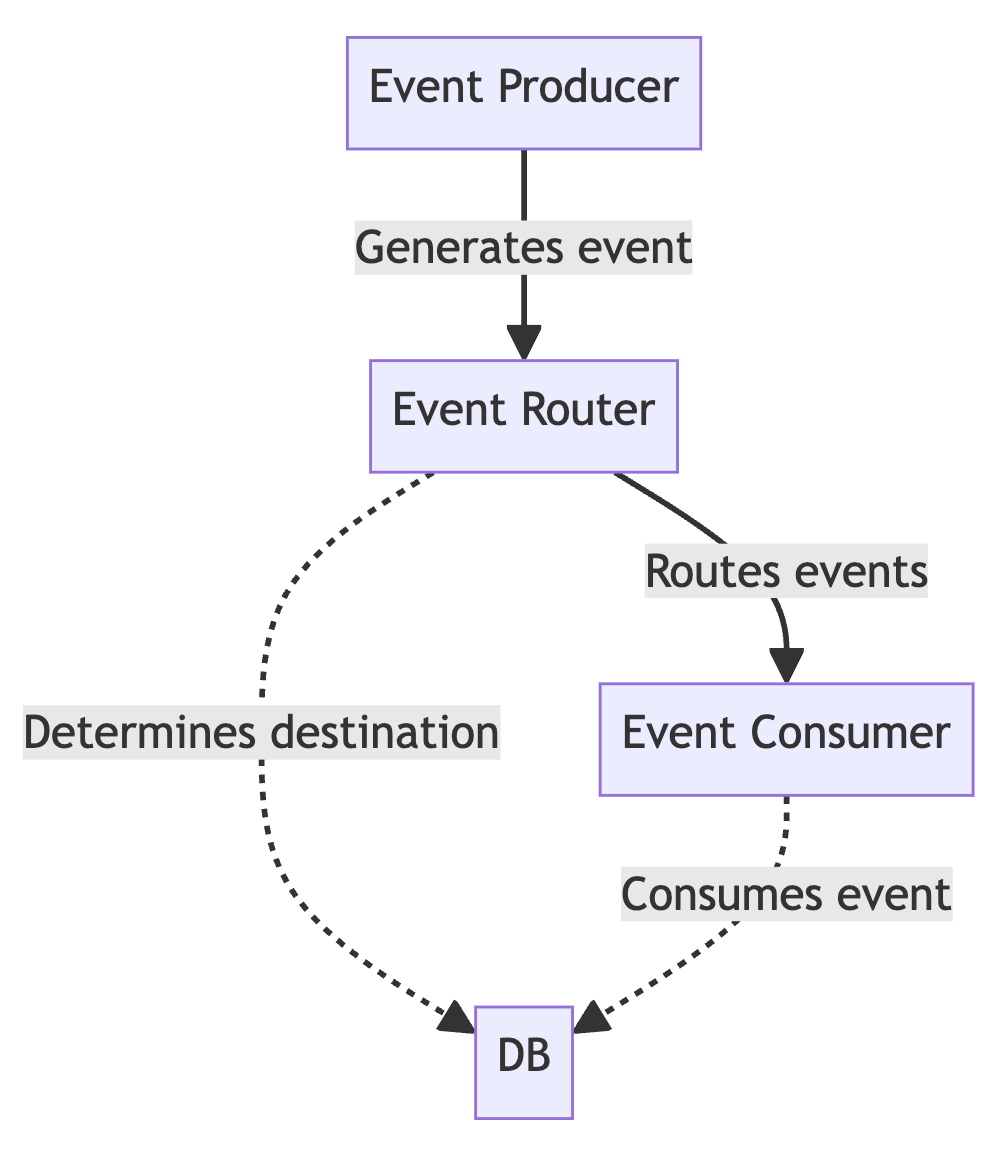
\includegraphics[width=70mm]{img/chap03/fig_event_driven_architecture_mermaid.png}
\caption{Event-Driven architecture diagram}
\label{img03:event_drive_architecture_diagram}
\end{figure}

%graph TD
%    Producer[Event Producer] -->|Generates event| Router[Event Router]
%    Router -->|Routes events| Consumer[Event Consumer]
%    Router -.->|Determines destination| DB
%    Consumer -.->|Consumes event| DB


\subsection{Client-Server architecture}
Client-server architecture divides system into two entities: clients who request services and servers that provide the services.
As stated in \cite{mediumArchitectureComparison} the functional characteristics of a client and a server are examples of programs that interact with each other within an application. The functionality of this architecture is highly flexible, as a single server can serve multiple clients as seen in Figure \ref{img03:client_server_architecture_diagram} or a single client can use multiple servers.
\begin{figure}[H]\centering
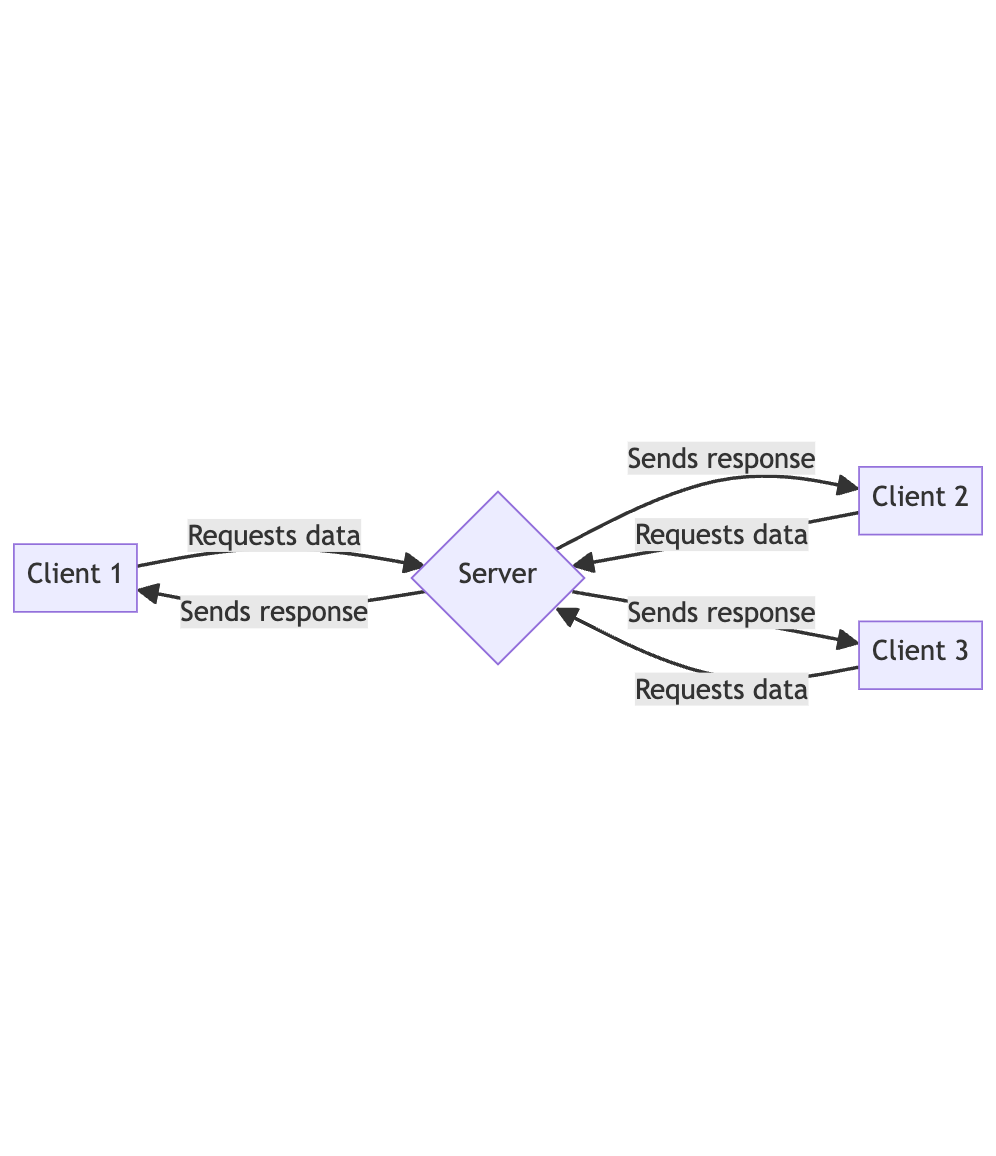
\includegraphics[width=80mm]{img/chap03/fig_client_server_architecture_mermaid.png}
\caption{Client-Server architecture diagram}
\label{img03:client_server_architecture_diagram}
\end{figure}

%graph TD
%    Producer[Event Producer] -->|Generates event| Router[Event Router]
%    Router -->|Routes events| Consumer[Event Consumer]
%    Router -.->|Determines destination| DB
%    Consumer -.->|Consumes event| DB

   

\subsection{Multi-Layer (N-Tier) architecture}
Multi-layer architecture, often referred to as n-tier, organises a system into logically separated layers that each handle specific types of processing as can be seen in Figure \ref{img03:multi_layer_architecture_diagram}. 
Typically, these include a presentation layer (user interface), an application layer (business logic), data layer, and database layer (data management). 
This separation helps better organization and allows for independent scaling, maintenance, or updating of each layer. 
Supports scalability and simplifies the development process by allowing teams to work on different layers independently.
\begin{figure}[H]\centering
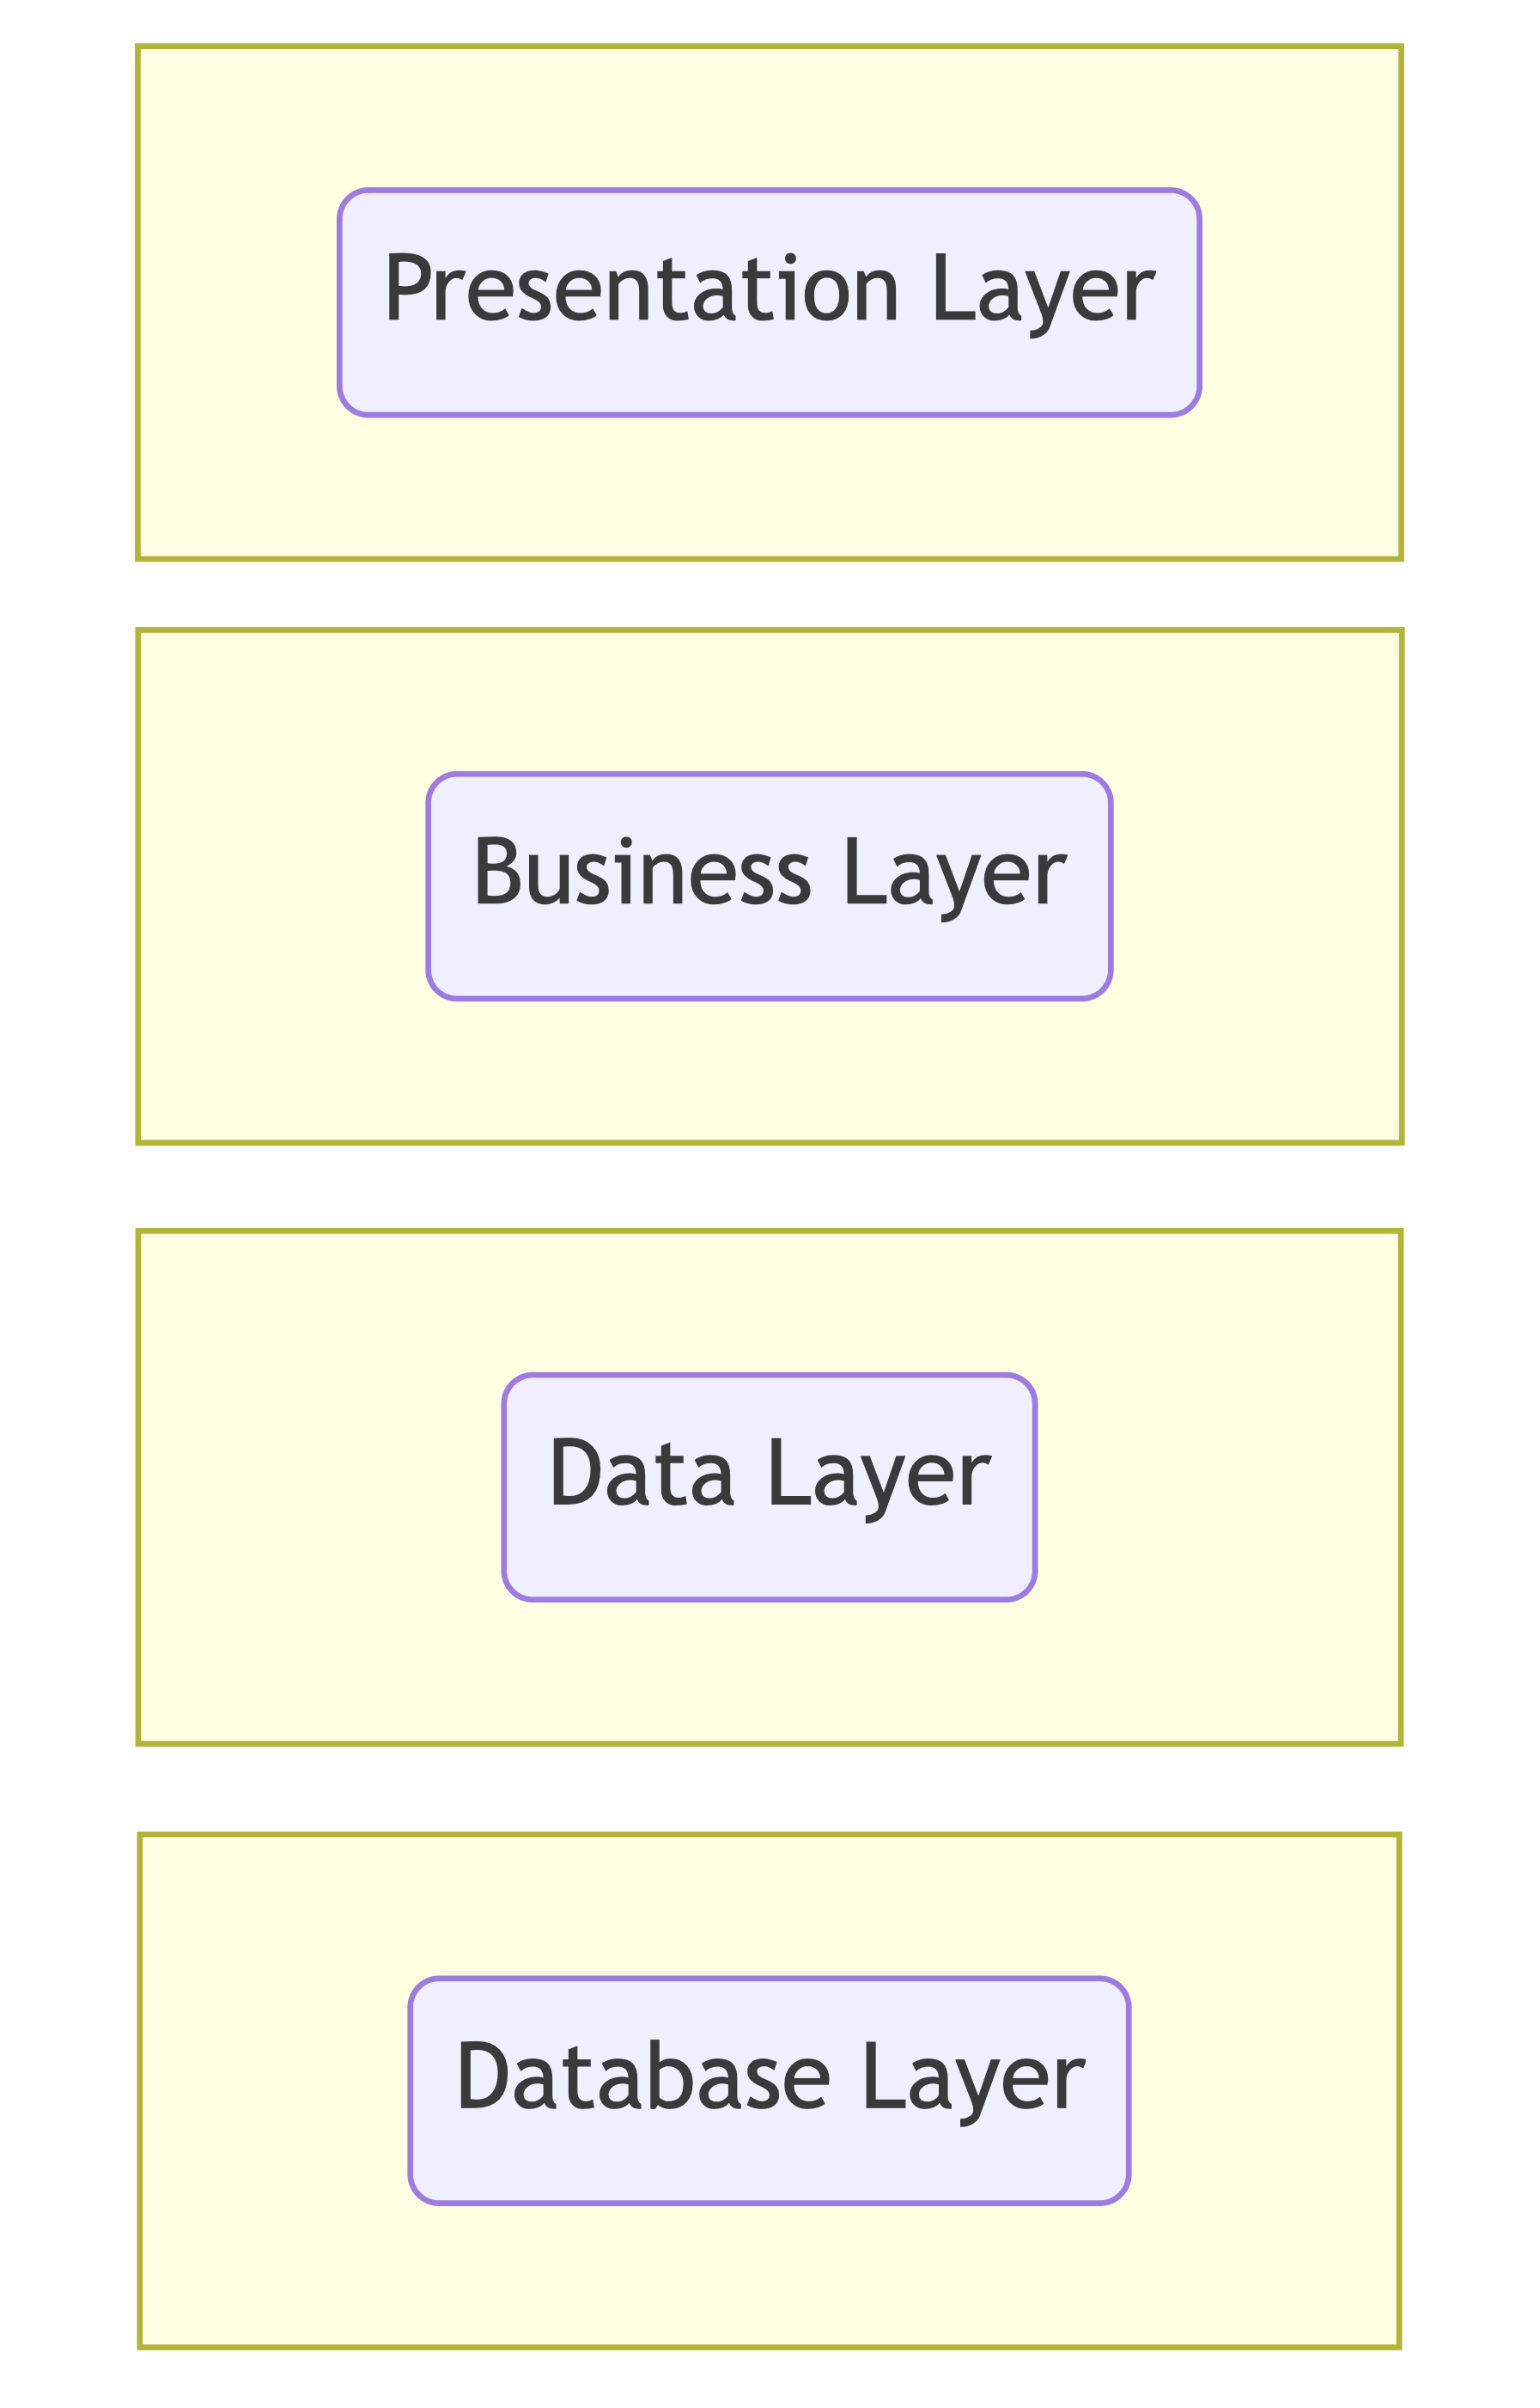
\includegraphics[width=60mm]{img/chap03/fig_multi_layer_architecture_mermaid.png}
\caption{Multi-Layer architecture diagram}
\label{img03:multi_layer_architecture_diagram}
\end{figure}

%graph TD;
% UI[User Interface] --> BL[Business Logic];
% BL --> DL[Data Storage];
% DL --> DS[Data Storage];

% subgraph UI_Layer[ ]
% 		UI(Presentation Layer)
% end

% subgraph BL_Layer[ ]
% 		BL(Business Layer)
% end

% subgraph DL_Layer[ ]
% 		DL(Data Layer)
% end

% subgraph DS_Layer[ ]
% 		DS(Database Layer)
% end

% style UI_Layer fill:##bdc3c7
% style BL_Layer fill:##bdc3c7
% style DS_Layer fill:##bdc3c7
% linkStyle default stroke-width:0;


\subsection{Comparison and selection}
Comparing these architectures, the event-driven architecture offers high responsiveness and is good for systems that require real-time capabilities due to its asynchronous capabilities.
The client-server model provides a robust architecture for handling interactions between centralised servers and multiple clients, which makes it suitable for traditional web applications. 
The multi-layer architecture offers flexibility in development and maintenance by separating concerns across multiple layers.

For our platform, the three-tier architecture, a specific form of multi-layer architecture, appears most suitable. This architecture divides the application into the presentation tier, logic tier, and data tier, which aligns well with our requirements for a scalable, maintainable system that can efficiently handle multiple user interactions and complex business processes. 
Additionally, this pattern complements our need for a multi-tenant environment.
Since the communication within layers is not cross-tier, we can support isolation between different tenant data.
The three-tier architecture as shown in Figure \ref{img03:layered_architecture_diagram} provides a balanced approach, offering a clear separation of concerns while maintaining simplicity in connectivity between the client and the server. 
It allows for efficient data processing and easier scalability management, as each layer can be scaled independently based on demand.

\begin{figure}[H]\centering
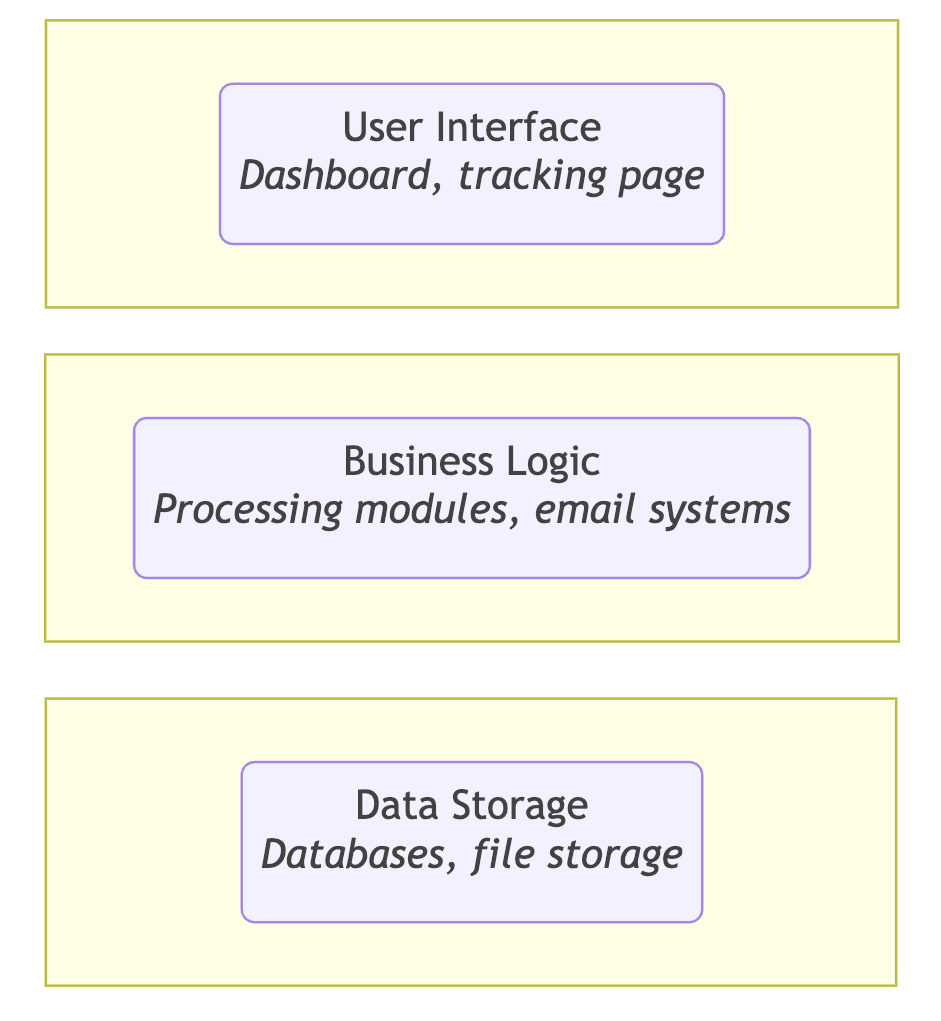
\includegraphics[width=80mm]{img/chap03/fig_layered_architecture_mermaid.png}
\caption{High-level layered architecture diagram}
\label{img03:layered_architecture_diagram}
\end{figure}


% graph TD;
%    UI[User Interface] --> BL[Business Logic];
%    BL --> DS[Data Storage];

%    subgraph UI_Layer[ ]
%        UI(User Interface<br><i>Dashboard, tracking page</i>)
%    end

%    subgraph BL_Layer[ ]
%        BL(Business Logic<br><i>Processing modules, email systems</i>)
%    end

%    subgraph DS_Layer[ ]
%        DS(Data Storage<br><i>Databases, file storage</i>)
%    end

%    style UI_Layer fill:##bdc3c7
%    style BL_Layer fill:##bdc3c7
%    style DS_Layer fill:##bdc3c7
%    linkStyle default stroke-width:0;
   
   

% Then present the image of the architecture  \ref{img03:c4_container_diagram_software_sytem} and describe it in detail and present how it will help solve the non-functional requirements

\section{System Architecture}
With the selection of a three-layer architecture as the most suitable model for our platform, we now present the architectural components proposed. 
This section outlines the high-level structure of the system, focusing on the main components and their roles without delving into detailed implementation specifics.
Let us take a look at the high-level diagram shown in Figure \ref{img03:c4_container_diagram_software_sytem} and describe the components shown in the figure.

\begin{figure}[H]\centering
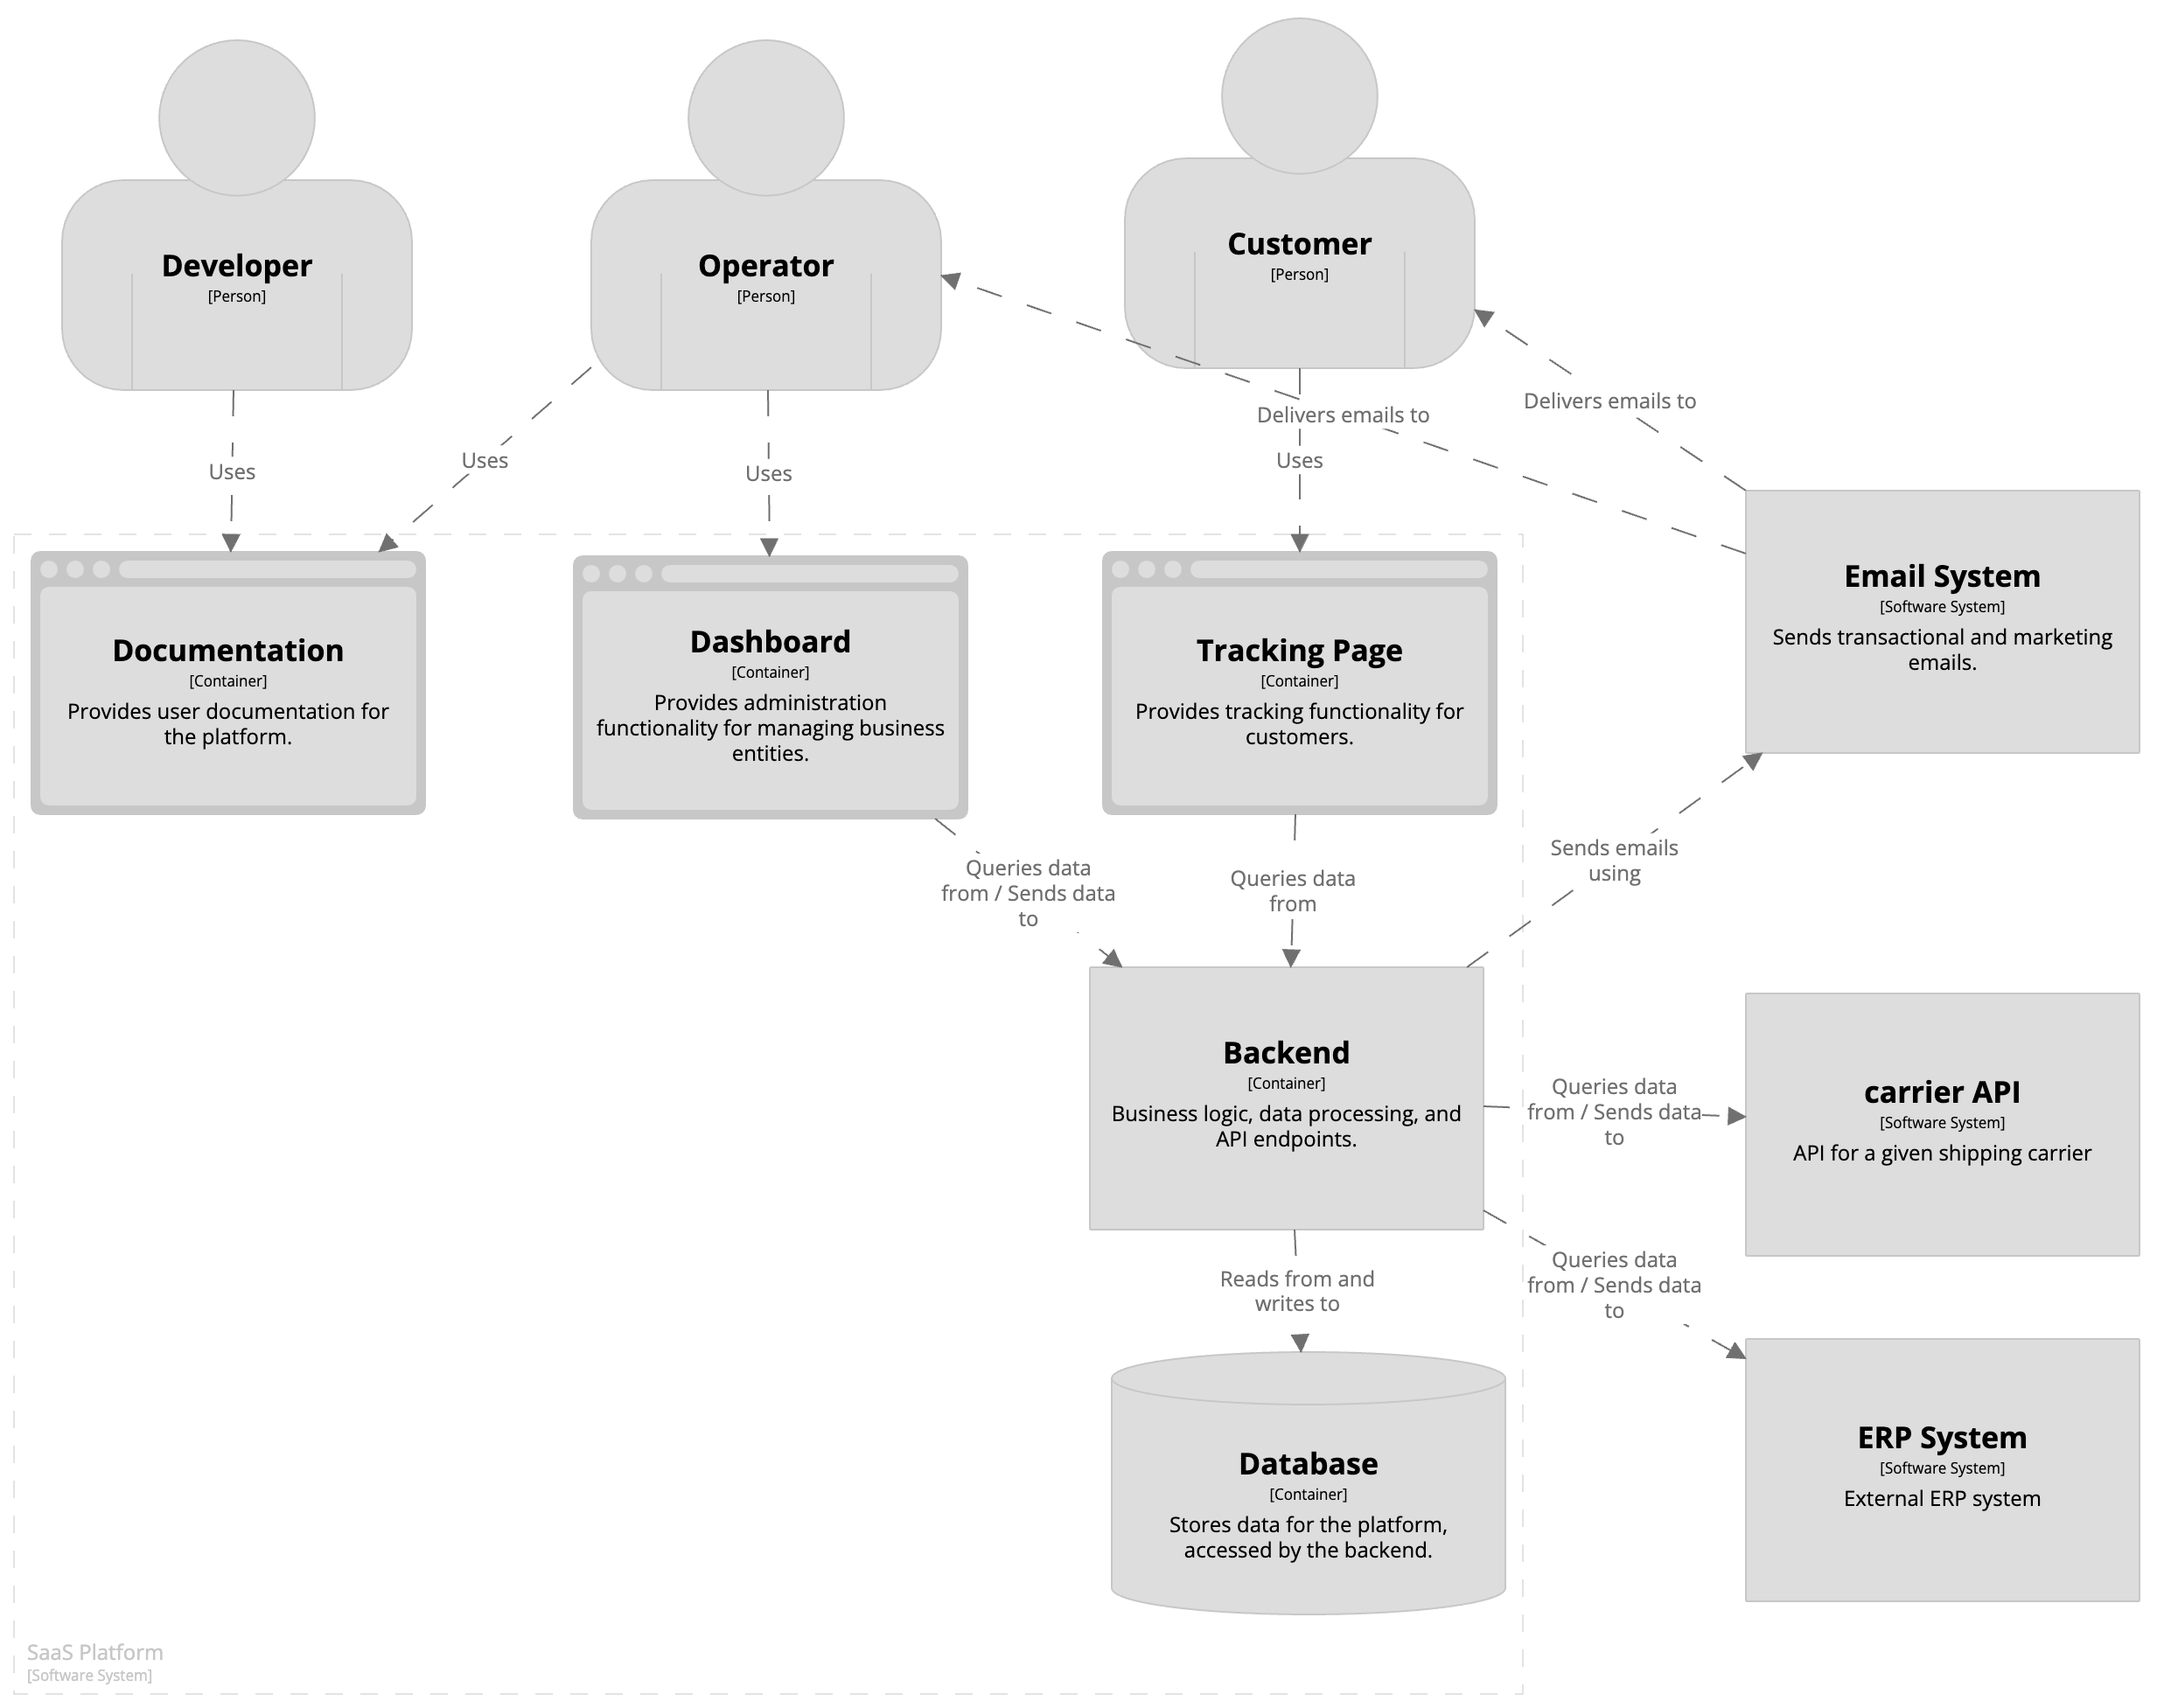
\includegraphics[width=140mm]{img/chap03/fig_architecture.png}
\caption{C4 container diagram of the software system}
\label{img03:c4_container_diagram_software_sytem}
\end{figure}

\subsection{Frontend Components}
The frontend of the platform consists of three main components, each serving a different purpose:

\begin{itemize}
    \item \textbf{Dashboard:} The central user interface for operators. 
    It enables operational management, including shipment tracking, carrier management, and analytics. 
    The dashboard is designed to be used primarily in desktop environments, but is responsive to be used on smaller screens.
    \item \textbf{Tracking Page:} An interface that allows end customers to track their shipments. 
    This page supports custom branding, allowing businesses to provide a cohesive brand experience. 
    Optimised for touch interaction, it improves accessibility and ease of use on mobile devices.
    \item \textbf{Docs:} A documentation website that provides users with guidelines, API documentation, and setup tutorials.
    This component is crucial for onboarding new Operators and supporting existing ones by offering easy access to necessary technical and usage information.
\end{itemize}

The backend serves as the core of the platform, integrating with external systems and APIs from shipping carriers, handling all data synchronisation tasks, shipment dispatch, and updates between the platform and shipping carriers. 
The business logic processes data from the frontend to ensure that all operations adhere to all business processes within our domain, which consists of shipment processing, user management, and the generation of customer notifications. 
In addition, an email system is integrated to manage communications with users by email based on specific triggers and events within the platform. 
This system is designed to support customizable email and tracking page templates, which allows for alignment with the branding requirements of different tenants, enhancing the customisation capability of the platform.

\subsection{Database}
The database serves as the central repository for storing all operational data along with user information. 
The database schema is designed to support multi-tenancy, implementing data isolation strategies that keep tenant data separate and secure. This setup is crucial in adhering to the multi-tenancy requirements of the architecture, ensuring that each tenant's data is accessed and managed securely without interference from or to other tenants.

\subsection{Overall System Interaction}
The frontend communicate with the backend via secure, REST API, which abstract the complexity of business processes and shipping carrier integrations.
The backend processes requests, interacts with the database for data retrieval and storage, and communicates with shipping carries or requests email notification sending.
It also opens another REST API for secure communication between the system and external services.

\section{Conclusion}
This architecture provides a blueprint for the development and operation of the platform. 
It supports the non-functional requirements outlined in the previous chapter \ref{subsec:nonfunctional-requirements}, such as scalability, maintainability, and extensibility, while also providing a flexible and user-friendly environment for both operators and customers.
All while being able to serve multiple tenants at the same time.